\chapter{Implementation}
\label{cha:impl}

Chapter 4

\section{Pre-Processing}

Figure \ref{bbdatatable} shows the raw format of the Britain Breathing dataset. There are a few procedures that need doing before it can be used in a hotspot identification algorithm. Before I had a web page running with the capability of displaying geographical data I relied on Tableau to visualise and alter all datasets.\\ 

The Britain Breathing dataset in it's raw format contained entries from all over the world. I could have decided to leave them on as I could centre the map on the UK so only those who where curious enough to pan around the rest of the globe would see these extra points. But that's more of a novel thing. At the time of pre-processing, I thought the extra points might affect some of the hotspot algorithm calculations such as global averages so I decided to remove all points that are not on mainland UK or in Northern and the Republic of Ireland.\\

\begin{SCfigure}
\label{fig:RTv1}
\caption{Figure \ref{fig:RTv1} : Britain Breathing dataset before processing}\\
\centering
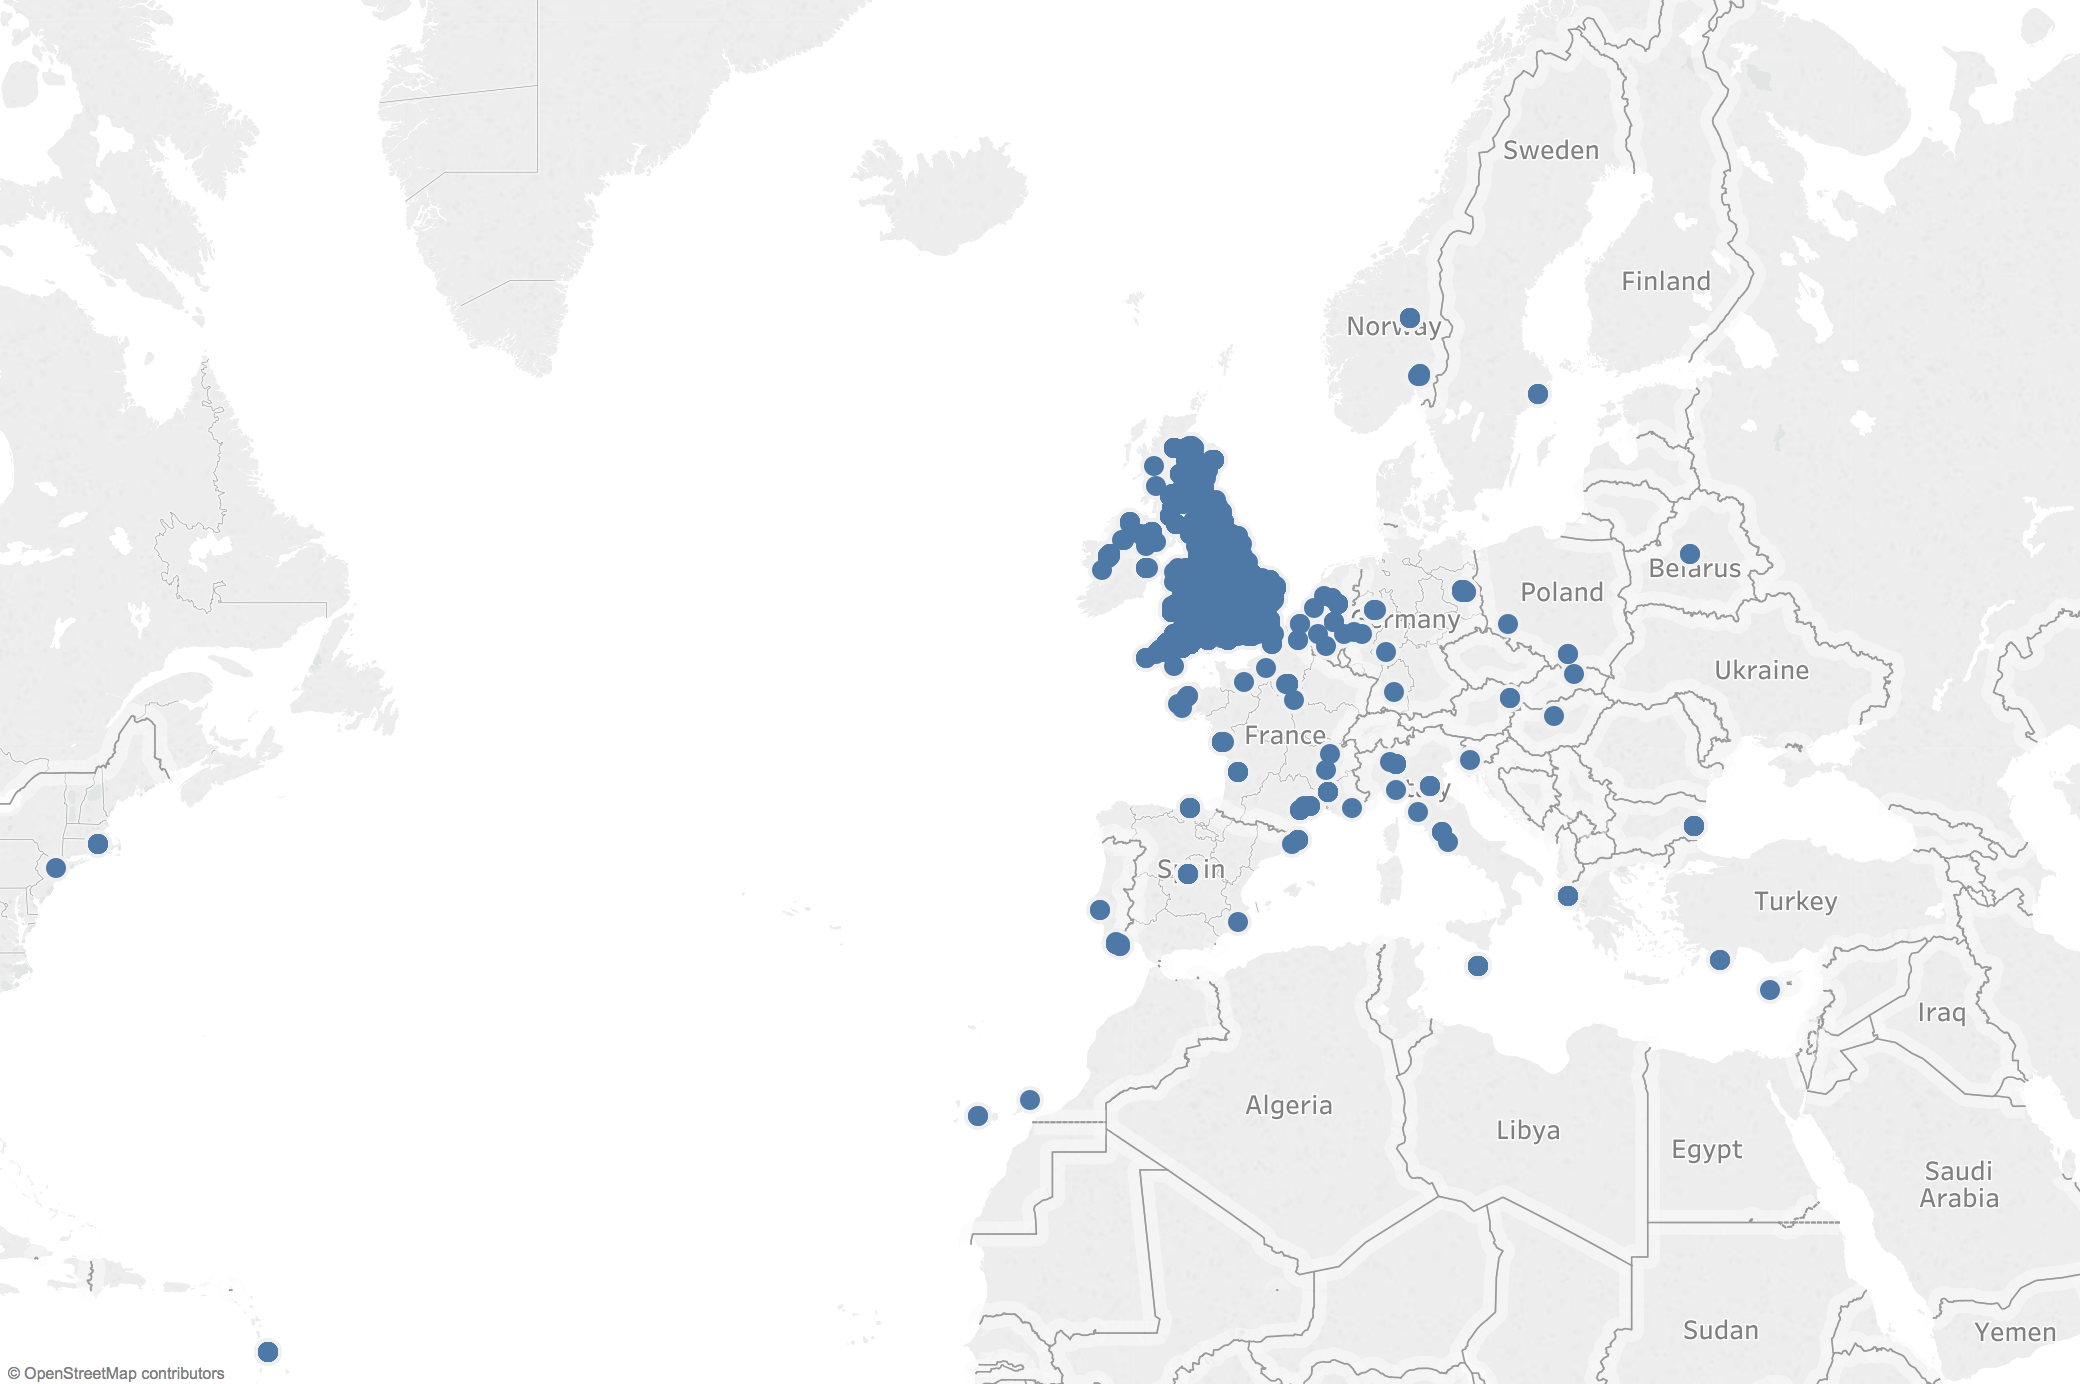
\includegraphics[width=0.75\textwidth]{tableuaeverywhere}
\centering
\end{SCfigure}\\

Approximately 2.7\% of entries had a null value for one of the attributes. 96\% of these nulls were  whether or not the user had existing hay fever or asthma, I decided to remove each of these records entirely, I could also have decided set the attribute to 0 or 1 but I wanted to avoid fabricating data to keep any conclusions made using the data valid.\\

Whilst using Tableau to visualise the data in the early stages of development I noticed there were a few clusters of points in virtually the same place. For example, there is a user in the north of Scotland who used the app at times multiple times a day to record her allergy symptoms. This resulted a fairly large set of results for a very sparsely populated area. I decided to remove most of the results for this person as the area was identified as a hotspot. I think there could be arguments for keeping the data but I don't think that allowing one persons enthusiasm to track her allergy problems makes sense for a project aimed at producing results that could be used to aid research.\\

Once the data has been improved from its raw format, it is stored on the server as a .JSON file. I decided against using a database to store my datasets as I wanted to avoid having to convert to and from JSON. The end application ended up being rather CPU intensive so this decision turned out very well.

\subsection{Road Traffic}

The Road Traffic dataset in its raw format was far from being usable.\\

As you can see from figure \ref{fig:rt} the first version of the Road Traffic dataset was way too dense. I needed the dataset to be able to be displayed with the heatmap generated from the Britain Breathing dataset to be visible behind the Road Traffic data in order to compare the two. There were too many roads of very short spans cluttering the view of the heatmap.\\

\begin{SCfigure}
\label{fig:rt}
\caption{Figure \ref{fig:rt} : First attempt at displaying the Road Traffic data}\\
\centering
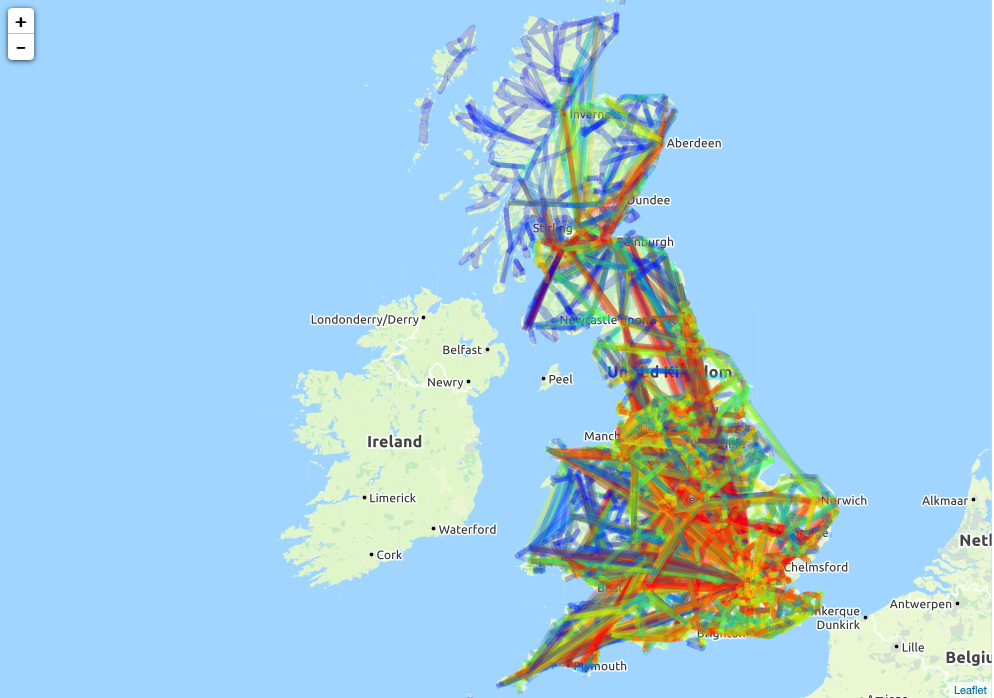
\includegraphics[width=0.75\textwidth]{RoadTrafficv1}
\centering
\end{SCfigure}\\

Upon zooming in and inspecting the data I also found that some roads were stored incorrectly in the dataset. Around 10 roads were stored as having their junction before and junction after being the ends of the road. Roads like the A1 can be as long as 396 miles so errors can cause big problems \cite{longestRoad}. In the case of the A1, the entire road was displayed as a deep red indicating a high volume of traffic. For the majority of the A1, this would be true but there are areas of the road that are not particularly busy so they're being wrongly represented. \\

I created a java program to process the data before being stored on the server. Java was chosen purely because I have most experience with it and I knew exactly how to read and write files, making it a good choice for pre-processing the Road Traffic data. For each entry, counts are discarded if the length of the distance between the junction before and the junction after is longer than 200km or if the road is shorter than 5km and has a density in the lower 5\% of the data. Removing the smaller roads like this removes the mess of small roads with negligable traffic in places like the north of Scotland. These roads don't provide much information and therefore do not help to find hotspots, they just make the map look cluttered.\\

\section{Heatmap Generation}

\subsection{Spatial AutoCorrelation}
\subsection{Getis-Ord}


\section{Allergy Score}

\section{Smart Data Tool}

Now that I have some good datasets and I understand how they effect each other, I need a way o

How relate dataset to specific allergies and symptoms